\chapter{Last Speech: Testimony, Scale, and the Work of Arrival}

This lecture has the structure of a farewell, but it does not behave like a mere farewell. It begins ceremonially, moves through affection and gratitude, then suddenly turns numerical and strategic. The thread that holds it together is testimony: first the testimony of one recovered body, then the testimony of a worldwide organization, and finally the testimony of countless small acts by which a culture reproduces itself. No validated mathematical screenshots survive for this lecture, so every displayed relation below is either directly transcript-backed or a cautious reconstruction stated as such. We shall follow the order of the talk itself: prologue, recovery, calculation, lag, arrival, place, testimony, apprenticeship, and closing charge.

\section{Prologue: Why Jim Rohn Matters Here}

The lecture opens with an emcee, and that is not an accident of stagecraft. Before Jim Rohn says anything substantial, the audience is told how to hear him. He is presented as continuous with Mark Hughes, not as an ornamental guest. The emcee explicitly says that the company is not doing anything different from the original dream, and that to understand the present one should go back and watch Mark.

That framing is followed by a personal anecdote. Some details in the transcript are garbled, but the secure line is clear enough: the emcee had worried about missing long-standing family Sundays, heard Rohn at an extravaganza, and came away feeling that this was not merely a motivational address but something like a spiritual event. The playful phrase about having gone to the ``church of Jim Rohn'' matters because it explains the scale of the introduction. Rohn is being introduced as a moral force within the history of the company.

Only after that does Rohn enter. He spends time greeting people, calling out friends, countries, and regions, and thanking the audience for its welcome. The room is allowed to become personal before it becomes analytical. That sequence is essential. A lecture about organization begins by making the organization visible as feeling and presence.

\begin{remark}
Because no validated frame-backed equations or diagrams survive for this lecture, the mathematics of the chapter must be carried by the transcript itself. The notes therefore distinguish between spoken numerical claims and compact editorial shorthand.
\end{remark}

\section{Recovery as Testimonial, Then Scale as Calculation}

Rohn's first genuine piece of evidence is bodily. He does not begin with market share, executive strategy, or even recruitment. He begins with illness. When he first became ill, he says, his weight had dropped to about \(123\) pounds. The recovery story is given in small, concrete steps:
\begin{align}
W_{\text{ill}} &\approx 123\ \text{lb},\\
s_{\text{ill}} &= 3\ \text{shakes/day},\\
\Delta W &> 30\ \text{lb},\\
s_{\text{later}} &= 2\ \text{shakes/day}.
\end{align}
The logic is not medical but testimonial. He was ill, he had little appetite, he took three shakes a day, he began gaining weight, he got better, and later he could cut back to two shakes a day. The gain of more than thirty pounds is not treated as a derivation; it is treated as witness.

The witness, however, does not remain private. Rohn immediately folds into the story the care of his daughter and Sarah, the letters and videos sent from around the world, and the claim that the audience's thoughts and prayers helped him recover. Then he turns that stream of care outward again. He says that his own prayers in the past year were for the audience: that they would be blessed with good people, that they would build a strong organization, that they would touch the people who needed to be touched. That is the real transition. Before he asks how large the market is, he first reminds us that scale matters only if it is tied to people.

Now the calculation appears. He asks Alan how many people are in the 70 countries. The intermediate estimate is verbally unstable, but the settled public claim is firm:
\begin{equation}
C = 70, \qquad M > 3\times 10^9,
\end{equation}
where \(C\) is the number of countries in which Herbalife is represented and \(M\) is the reachable market.

\begin{table}[h]
\centering
\begin{tabular}{p{0.42\linewidth} p{0.30\linewidth}}
weight at the worst stage of illness & \(W_{\text{ill}} \approx 123\ \text{lb}\) \\
shakes during illness & \(3\ \text{shakes/day}\) \\
later maintenance level & \(2\ \text{shakes/day}\) \\
weight regained & \(>30\ \text{lb}\) \\
countries represented & \(70\) \\
reachable market & \(>3\times 10^9\) people \\
illustrative income floor & \(\$1/\text{day}\) \\
large meeting scale & \(18{,}000\) people
\end{tabular}
\caption{Transcript-backed numerical anchors for the lecture.}
\end{table}

\subsection{Question \& Answer}

Why does the lecture move from one person's recovery to a market of billions?

Because Rohn uses testimony as a local proof that then demands enlargement. The recovery story is not there merely to humanize him. It establishes that products, people, and prayers have produced a visible effect in one life. Once that is admitted, the next question is unavoidable: how many people still stand outside such a transformation? The transition to 70 countries and more than 3 billion people is therefore not an imported business statistic; it is the scaling-up of the testimonial itself.

\section{The Market Is Vast, and We Are Still Behind}

Once the number \(M>3\times 10^9\) has been put on the table, one expects a pause for self-congratulation. Rohn does the opposite. He says, in effect, so guess what: we are behind. This is the lecture's first serious conceptual obstacle. How can an organization be in 70 countries, face a market of billions, be meeting in vast halls, and still honestly describe itself as behind?

His sharpest formulation is intentionally colloquial:
\begin{equation}
1\ \text{new customer} \mapsto 3\ \text{new babies}.
\end{equation}
This is not literal demography. It is the lecture's rate comparison in memorable form. In cautious mathematical shorthand, the point is
\begin{equation}
r_{\text{need}} > r_{\text{reach}},
\end{equation}
so that the service gap
\begin{equation}
\Delta(t)=N_{\text{market}}(t)-N_{\text{served}}(t)
\end{equation}
does not automatically shrink just because the organization is busy.

\paragraph{A one-step model.}
If we sample that logic at discrete moments and let \(\Delta_n\) denote the gap at step \(n\), then the slogan ``one customer, three babies'' becomes the update
\begin{equation}
\Delta_{n+1}=\Delta_n+3-1=\Delta_n+2.
\end{equation}
The arithmetic is elementary, but the conclusion is severe: the organization may be genuinely growing while the unmet field grows faster still.

Later in the talk Rohn gives the same argument in historical form. After 29 years in America, he says, there are more overweight people than when they started. In the spirit of the lecture, we may record the judgment as
\begin{equation}
N_{\text{overweight,US}}(29\ \text{years later}) > N_{\text{overweight,US}}(0).
\end{equation}
Again the point is not statistical proof in a strict economic sense. The point is structural lag. As fast as we run, we may still remain behind if the need keeps widening.

\begin{figure}[h]
\centering
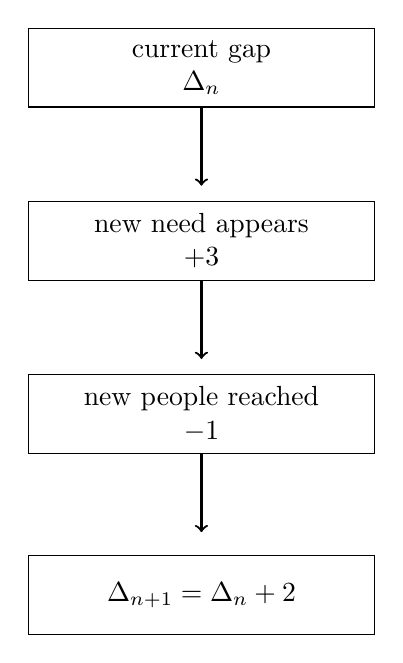
\begin{tikzpicture}[x=1cm,y=1cm]
\draw (0.3,7.2) rectangle (4.7,8.2);
\node[align=center] at (2.5,7.7) {current gap\\\(\Delta_n\)};

\draw[->, thick] (2.5,7.2) -- (2.5,6.2);

\draw (0.3,5.0) rectangle (4.7,6.0);
\node[align=center] at (2.5,5.5) {new need appears\\\(+3\)};

\draw[->, thick] (2.5,5.0) -- (2.5,4.0);

\draw (0.3,2.8) rectangle (4.7,3.8);
\node[align=center] at (2.5,3.3) {new people reached\\\(-1\)};

\draw[->, thick] (2.5,2.8) -- (2.5,1.8);

\draw (0.3,0.5) rectangle (4.7,1.5);
\node[align=center] at (2.5,1.0) {\(\Delta_{n+1}=\Delta_n+2\)};
\end{tikzpicture}
\caption{Transcript-only schematic of the lecture's lag model: new need outruns current reach.}
\end{figure}

\subsection{Question \& Answer}

Why can a rapidly growing organization still say that it is behind?

Because growth is not the same thing as closure. Rohn's distinction is between doing much work and catching up to the size of the field. If new need enters faster than the organization reaches new people, then busyness and insufficiency coexist. The lecture is careful here. ``We're behind'' is not a mood. It is a quantitative judgment about the difference between the growth of need and the growth of reach.

\section{Mission, Management, and Mark's Dream of a Place}

Having defined lag, the lecture next refuses to leave it at the level of abstract arithmetic. Rohn translates the market into a waiting population. The repeated phrase is ``until you get there.'' Until you get there, people remain overweight; until you get there, health problems remain; until you get there, in some places people are earning only
\begin{equation}
I_{\min}=\$1/\text{day}.
\end{equation}
Until you and your organization arrive---knocking on the door, handing out a flyer, saying hello---the economic and personal condition stays unchanged.

In compact editorial shorthand, the logic may be written as
\begin{equation}
\text{organizational arrival} \to \{\text{health},\ \text{income},\ \text{recognition}\}.
\end{equation}
One should read that cautiously. The lecture itself is not building a formal social model. It is insisting on causality in plain language: nothing changes for many people until somebody arrives with products, story, welcome, and opportunity.

From here Rohn praises Michael Johnson. He says he does not know how a CEO manages to keep all the products flowing into 70 countries. The name of the job, he jokes, is ``impossible.'' That praise is not decorative. It prepares the next inference: if the executive task is already impossible, then the burden of the mission must be carried by the field of distributors itself.

The lecture then narrows the question. What sort of thing did Mark Hughes want to build? A room is a place. A hotel is a place. But the real place is something else.

\begin{definition}
In the logic of this lecture, a \emph{place} is not merely an enclosure. It is a human field made of distributors, stories, products, invitation, memory, and return.
\end{definition}

Rohn tracks that enlargement historically. Mark opened the first 50 countries; Michael added roughly 20 more:
\begin{align}
50 + 20 &= 70,\\
N_{\text{meeting}} &= 18{,}000.
\end{align}
The second number matters because he later recalls large gatherings, including the Mexico extravaganza he regretted missing, as evidence that the ``family place'' has expanded far beyond a small room. Yet even now the lecture insists on the same conclusion: the place is the people, the distributors, you and me.

\subsection{Question \& Answer}

What is the ``place'' that Herbalife is meant to create?

Not first a venue. Not first a hotel ballroom. The place is the organized human environment in which people hear a story, use the products, improve their health, bless their families, start earning money, and are recognized by others. Once we see that, a large meeting of \(18{,}000\) is not merely an event statistic. It is evidence that the place has become portable, reproducible, and global.

\section{Training and Testimonials: Head and Heart}

Once the place has been defined, Rohn turns to the mechanism that operates within it. Here the lecture becomes unusually explicit. The phrase to master is ``the testimonials.'' But the testimonials do not replace training. They accompany it. The two channels are sharply distinguished:
\begin{align}
\text{training} &\to \text{head},\\
\text{testimonials} &\to \text{heart}.
\end{align}
In editorial shorthand we may state the same point as
\begin{equation}
\text{training} \to \text{understanding}, \qquad
\text{testimonials} \to \text{motivation}.
\end{equation}

This is not just rhetorical polish. It is a genuine pedagogical structure. Training gives answers, information, and clarity. Testimonials show that the information has already entered a life. That is why the lecture keeps reaching for early examples: ``here is what has happened to my health,'' ``here is what has happened to my family,'' ``I have started making money already.'' The compact map is
\begin{equation}
\text{Herbalife participation} \to \{\text{health},\ \text{family},\ \text{income}\}.
\end{equation}

Rohn then folds the organizational horizon back into this same point. The company is in 70 countries, serving more than 3 billion people, and in his aspirational language that scale is moving onward:
\begin{equation}
3\times 10^9 \to 4\times 10^9 \to 5\times 10^9.
\end{equation}
One should not read that as a forecast. In the lecture it functions as a motivational horizon. Training has already made large-scale expansion possible; testimonials are what keep the expansion human.

The historical example of the Little London meetings growing into Royal Albert Hall serves exactly this purpose. The enlargement of the room is itself a testimonial. The venue is not being admired for its architecture. It is being cited as evidence that the story has already been lived, retold, and multiplied.

\begin{table}[h]
\centering
\begin{tabular}{p{0.28\linewidth} p{0.28\linewidth}}
training & testimonials \\
head & heart \\
information & felt proof \\
answers & motivation \\
understanding & desire to join and stay
\end{tabular}
\caption{The lecture's two-channel persuasive structure.}
\end{table}

\subsection{Question \& Answer}

Why are both training and testimonials necessary?

Because the lecture does not trust explanation by itself, and it does not trust emotional lift by itself. Training without testimony may leave a person informed but untouched. Testimony without training may leave a person moved but ungrounded. Rohn's structure is therefore two-step: let people understand, and let them feel; let the head be reached, and let the heart be reached. Only then can the organization expand without becoming hollow.

\section{Always Say Yes: The Small-Scale Algorithm of Leadership}

The final major movement of the lecture is a descent from planetary scale to the smallest repeatable action. We have been talking about 70 countries and 3 billion people; now Rohn asks what the beginner should do in a room tonight. The answer is as simple as it is insistent: always say yes.

If someone asks you to participate in a meeting, give your testimonial, stand by the door, shake hands with brand-new people, welcome those who are just arriving, say yes. This is not merely politeness. It is apprenticeship. Leadership begins below the level of formal leadership.

The ladder may be written as
\begin{equation}
\text{say yes to small tasks} \to \text{hospitality} \to \text{testimonial} \to \text{leadership}.
\end{equation}

\paragraph{A practical update rule.}
The lecture's sequence may be rendered as a small iterative discipline:
\begin{enumerate}
\item accept the public task that is offered;
\item learn to welcome and steady the room;
\item speak when asked, even briefly;
\item encourage the person who is brand new;
\item grow into the ability to train others.
\end{enumerate}

This explains why Rohn says that leadership training is not only learning to give a good training program. It is learning to shake hands, learning to say hello, learning to say welcome. The culture of Herbalife is reproduced through these little acts before it is ever formalized as instruction.

The same stretch of the lecture carries several compressed promises: tell the newcomer that he is going to hear a fantastic story; tell him he is going to make it; if he says that after four days he has made no sales, tell him the fifth day is the magic day; if last week was difficult, tell him next week may be his best week ever. These are not detachable pieces of optimism. They are the spoken operating code of a culture that wants to keep beginners moving.

Rohn then gathers the strands one last time. Remember Mark Hughes. Remember the simple story. Remember the testimonials. Remember the challenge. We are still behind, and therefore we must run to catch up as best we can. The closing gratitude to Sarah, to his daughter, to the home office staff, to those who filled in for him when he could not travel, belongs to the same structure. The farewell is not a retreat from mission. It is mission voiced under the pressure of frailty.

The lecture therefore ends not in resignation but in renewed acceleration: we are fulfilling Mark's dream; after 29 years there is still more work to do; let us grow, accelerate, expand, reach out, and touch somebody with what we have.

\subsection{Question \& Answer}

What does leadership training look like before one is ready to teach?

It looks like disciplined assent to visible, ordinary duties. The lecture does not place leadership behind mystery or talent. It begins with yes: yes to the door, yes to the handshake, yes to the welcome, yes to the testimonial, yes to the room. Large organization is built out of these small and repeated permissions.

\section{Summary}

The lecture begins with an introduction, but its real shape is a chain of enlargements. A body recovers. That recovery becomes testimony. Testimony becomes a market calculation. The market calculation becomes a paradox of lag. The paradox becomes a mission of arrival. Arrival becomes a human place. Inside that place, training reaches the head, testimonials reach the heart, and leadership begins in the first small yes.

What makes the lecture powerful is that it never lets the numbers float free from the people. \(70\) countries and more than \(3\times 10^9\) people are not trophies; they are measures of unfinished work. Even the farewell obeys that law. Gratitude, illness, prayer, affection, and blessing are all folded back into a final imperative: the dream is still alive, the field is still larger than the reach, and therefore the work must continue.